\chapter {Interfacing a Servomotor}
\thispagestyle{empty}
\label{sec:servo}
\newcommand{\LocSERfig}{\Origin/user-code/servo/figures}
\newcommand{\LocSERscicode}{\Origin/user-code/servo/scilab}
\newcommand{\LocSERscibrief}[1]{{\tt \seqsplit{%
        Origin/user-code/servo/scilab/#1}},
  see \fnrefp{fn:file-loc}}

\newcommand{\LocSERardcode}{\Origin/user-code/servo/arduino}
\newcommand{\LocSERardbrief}[1]{{\tt \seqsplit{%
        Origin/user-code/servo/arduino/#1}},
  see \fnrefp{fn:file-loc}}

%%%%%%%%%%%%%%%python starts
\newcommand{\LocSERpycode}{\Origin/user-code/servo/python}
\newcommand{\LocSERpybrief}[1]{{\tt \seqsplit{%
        Origin/user-code/servo/python/#1}},
  see \fnrefp{fn:file-loc}}
%%%%%%%%%%%%%%%python ends

%%%%%%%%%%%%%%%julia starts
\newcommand{\LocSERjuliacode}{\Origin/user-code/servo/julia}
\newcommand{\LocSERjuliabrief}[1]{{\tt \seqsplit{%
        Origin/user-code/servo/julia/#1}},
  see \fnrefp{fn:file-loc}}
%%%%%%%%%%%%%%%julia ends

%%%%%%%%%%%%%%% OpenModelica starts
\newcommand{\LocSEROpenModelicacode}{\Origin/user-code/servo/OpenModelica}
\newcommand{\LocSEROpenModelicabrief}[1]{{\tt \seqsplit{%
        Origin/user-code/servo/OpenModelica/#1}},
  see \fnrefp{fn:file-loc}}
%%%%%%%%%%%%%%% OpenModelica ends

A servomotor is a very useful industrial control mechanism.  Learning
to control it will be extremely useful for practitioners.  In this
chapter, we will explain how to control a servomotor using the
\arduino\ board.  We will begin with preliminaries of servomotors and
explain how to connect a typical servomotor to the \arduino\ board and
shield.  We will then explain how to control it through the Arduino IDE,
Scilab scripts, Scilab Xcos, Python, Julia, and OpenModelica. 
We will provide code for all the experiments.

\section{Preliminaries}
\label{sec:servo-pril}
A servomotor is a rotary control mechanism.  It can be commanded to
rotate to a specified angle.  It can rotate in positive or negative
direction.  Using servomotors, one can control
angular position, velocity and acceleration.  Servomotors are useful
in many applications.  Some examples are robotics, industrial motors
and printers.

Typical servomotors have a maximum range of $180^\circ$, although some
have different ranges\footnote{All the angles in a servomotor are
  absolute angles, with respect to a fixed reference point, which can
  be taken as $0^\circ$.}.
Servomotors typically have a position sensor,
using which, rotate to the commanded angle.  The minimum angle to
which a servomotor can be rotated is its least count, which varies
from one model to another.  Low cost servomotors have a large least
count, say, of the order of $10^\circ$.

A servomotor typically comes with three terminals for the
following three signals: position signal, Vcc and ground. 
Position signal means that this terminal should be connected to 
one of the PWM (Pulse Width Modulation) pins \cite{arduino-pwm} on \arduino. 
This book uses PWM pin 5 for this purpose. 
Rest two terminals (Vcc and ground) need to be connected to 5V and GND on \arduino. 
\tabref{tab:servo-connect} summarizes these connections. 

We now explain how to connect a typical servomotor to the shield attached 
on the \arduino\ board. On the shield, there is a three-pin header at one of the 
ends. The pins of this header have been marked as $1$, $2$, and $3$. These pins:
$1$, $2$, and $3$ are internally connected to 5V, PWM pin 5, and GND on \arduino\, respectively.  
As discussed before, a typical servomotor has three terminals. Thus, the readers need to 
connect these three terminals with the three-pin header, as shown in \figref{fig:servo-shield}
before running the experiments given in this chapter. 

\begin{figure}
  \centering
  \includegraphics[width=\lgfig]{\LocSERfig/servo-uno-shield.jpg}
  \caption{Connecting servomotor to the shield attached on \arduino}
  \label{fig:servo-shield}
\end{figure}


\begin{table}
  \centering
  \caption{Connecting a typical servomotor to \arduino\ board}
  \label{tab:servo-connect}
  \begin{tabular}{lc}\hline
    Servomotor terminal                & Arduino board \\ \hline
    Position signal (orange or yellow) & 5             \\
    Vcc (red or orange)                & 5V            \\
    Ground (black or brown)            & GND           \\ 
    \hline
  \end{tabular}
\end{table}


\section{Connecting a servomotor with \arduino\ using a breadboard}
This section is useful for those who either don't have a shield or don't want to use the shield
for performing the experiments given in this chapter. 

A breadboard is a device for holding the components of a circuit and connecting 
them together. We can build an electronic circuit on a breadboard without doing any 
soldering. To know more about the breadboard and other electronic components, 
one should watch the Spoken Tutorials on Arduino as published on
  {\tt https://spoken-tutorial.org/}. Ideally, one should go through all the
tutorials labeled as Basic. However, we strongly recommend the readers should
watch the fifth and sixth tutorials, i.e., {\tt First Arduino Program} and 
  {\tt Arduino with Tricolor LED and Push button}.

In case you have a servomotor and want to connect it with \arduino\ on a breadboard, 
please refer to \figref{fig:servo-bread}. 
\begin{figure}
  \centering
  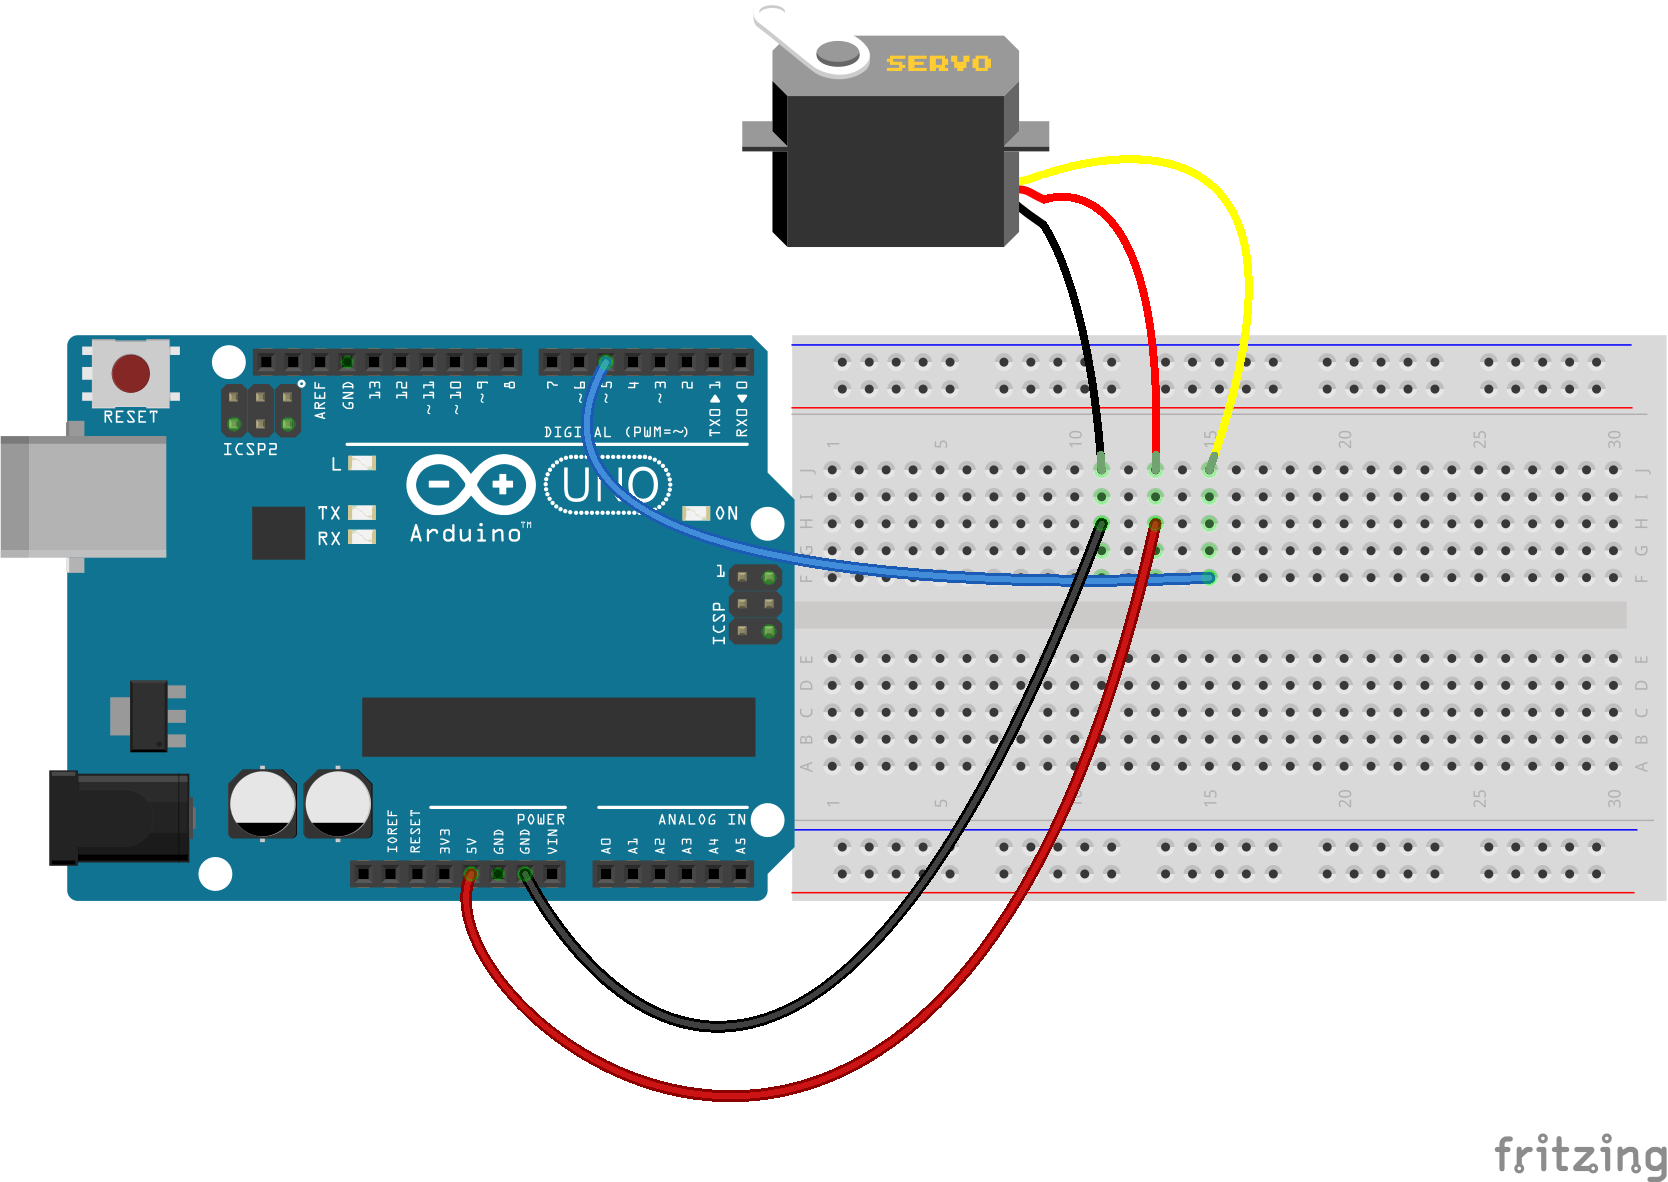
\includegraphics[width=\hgfig]{\LocSERfig/servo-bb.png}
  \caption{A servomotor with \arduino\ using a breadboard}
  \label{fig:servo-bread}
\end{figure}
As shown in \figref{fig:servo-bread}, there is a servomotor with three 
terminals. These terminals are used for the same three signals, as that explained 
in \secref{sec:servo-pril}. The connections shown in \figref{fig:servo-pot-bread} can 
be used to control the position of the servomotor, depending on the 
values coming from a potentiometer. As shown in \figref{fig:servo-pot-bread}, 
analog pin 2 on \arduino\ is connected to the middle leg of the 
potentiometer. Rest of the connections are same as that in \figref{fig:servo-bread}. 

\begin{figure}
  \centering
  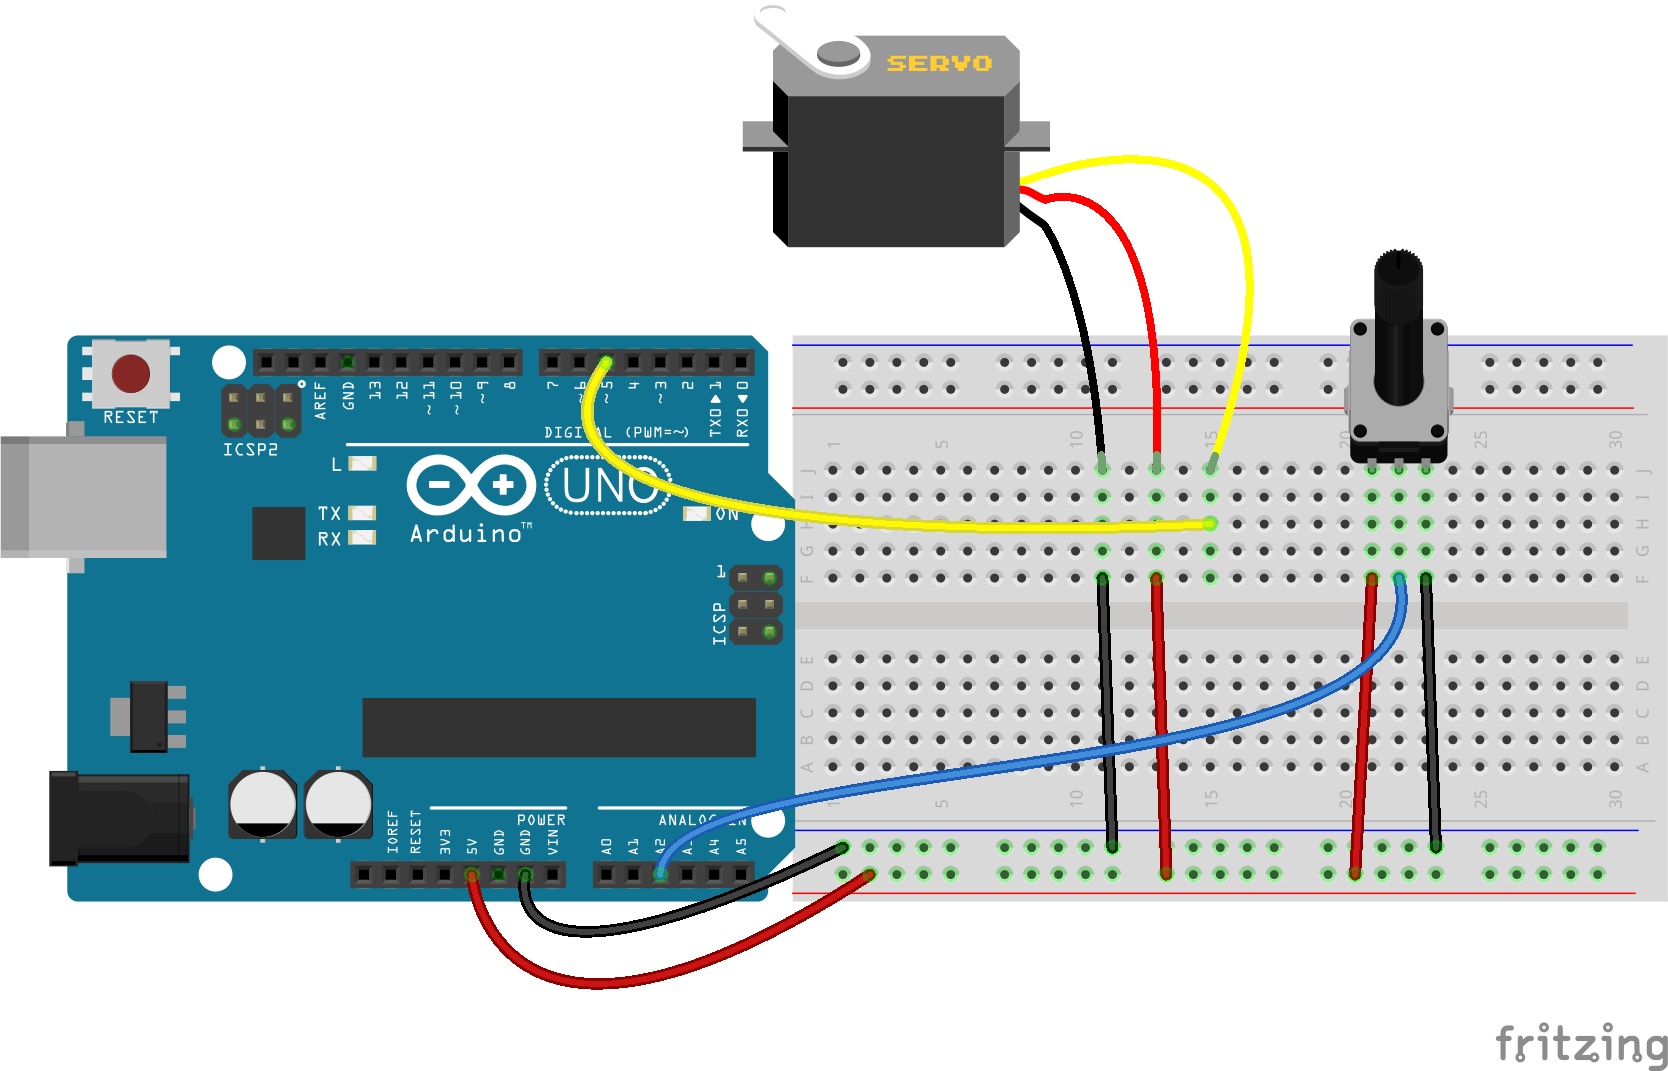
\includegraphics[width=\hgfig]{\LocSERfig/servo-pot-bb.png}
  \caption{A servomotor and a potentiometer with \arduino\ using a breadboard}
  \label{fig:servo-pot-bread}
\end{figure}

\section{Controlling the servomotor through the Arduino IDE}
\subsection{Controlling the servomotor}
\label{sec:servo-ard}
In this section, we will describe some experiments that will help
rotate the servomotor based on the command given from Arduino IDE.  We
will also give the necessary code.  We will present four experiments
in this section.  The shield has to be attached to the \arduino\ board
before doing these experiments and the \arduino\ needs to be connected to the computer 
with a USB cable, as shown in \figref{arduino}. The reader should go through the
instructions given in \secref{sec:ard-start} before getting started.

\begin{enumerate}
  %\setcounter{enumi}{-1}
  \item In the first experiment, we will move the servomotor by
        $30^\circ$. \ardref{ard:servo-init} has the required code for this.  
        This code makes use of a library named {\tt Servo} \cite{servo-lib}. 
        Thus, we include its header file at the top of \ardref{ard:servo-init}:
        \lstinputlisting[firstline=1,lastline=1]
        {\LocSERardcode/servo-init/servo-init.ino}
        Next, we create a {\tt Servo} object and call it {\tt myservo}, as shown below:
        \lstinputlisting[firstline=2,lastline=2]
        {\LocSERardcode/servo-init/servo-init.ino}
        Most Arduino boards allow the creation of 12 servo objects. Next, we initialize the port for serial communication at
        data rate of 115200 bits per second. Following to this, we mention the 
        pin to which the servo is attached, as shown below:
        \lstinputlisting[firstline=5,lastline=5]
        {\LocSERardcode/servo-init/servo-init.ino}
        With this, we issue the command to rotate the servomotor by $30^\circ$ followed by a delay of 
        1000 milliseconds:
        \lstinputlisting[firstline=6,lastline=7]
        {\LocSERardcode/servo-init/servo-init.ino}
        At last, we  detach the servomotor.    
        
        Once this code is executed, the servomotor would move by
        $30^\circ$, as commanded.  What happens if this code is executed
        once again?  The motor will not move at all.  What is the reason?
        Recall that what we assign to the motor are absolute positions, with
        respect to a fixed origin.  As a result, there will be no change at
        all. 
        
  \item In the second experiment, we move the motor by $90^\circ$ in the
        forward direction and $45^\circ$ in the reverse direction.  This
        code is given in \ardref{ard:servo-reverse}.  In this code, 
        we have added a delay of 1000 milliseconds between the two instances of 
        rotating the servomotor: 
        \lstinputlisting[firstline=6,lastline=8]
        {\LocSERardcode/servo-reverse/servo-reverse.ino}
        What is the reason behind this delay?  If the delay were not
        there, the motor will move only by the net angle of $90-45 = 45$
        degrees.  The reader should verify this by commenting on the delay
        command.
        
  \item In the third experiment, we move the motor in increments of
        $20^\circ$.  This is achieved by the {\tt for} loop, as in
        \ardref{ard:servo-loop}.  Both {\tt i}, the loop variable and {\tt
            angle}, the variable to store angle, are declared as {\tt int} in
        this code.  The code helps the motor move in steps of $20^\circ$ all
        the way to $180^\circ$.  
        
  \item Finally, in the last experiment, we read the potentiometer value
        from the shield and use it to drive the servomotor, see
        \ardref{ard:servo-pot}.  The resistance of the potentiometer is
        represented in 10 bits.  As a result, the resistance value could be
        any one of 1024 values, from 0 to 1023.  This entire range is
        mapped to $180^\circ$, as shown below:
        \lstinputlisting[firstline=10,lastline=12]
        {\LocSERardcode/servo-pot/servo-pot.ino}
        By rotating the potentiometer, one can make
        the motor move by different amounts.
        
        As mentioned in \chapref{potmeter}, the potentiometer on the shield is connected 
        to analog pin 2 on \arduino. Through this pin, the resistance of the potentiometer, in the range of 0 to 1023,
        depending on its position, is read.  Thus, by rotating the
        potentiometer, we make different values appear on pin 2.  This value
        is used to move the servo.  For example, if the resistance is half
        of the total, the servomotor will go to $90^\circ$ and so on.  The
        servomotor stops for 500 milliseconds after every move.  The loop is
        executed for 50 iterations. During this period, the servomotor keeps moving as dictated by the
        resistance of the potentiometer. While running this experiment, the readers 
        must rotate the knob of the potentiometer and observe 
        the change in the position (or angle) of the servomotor.   
        
\end{enumerate}

\begin{exercise}
  Let us carry out this exercise:
  \begin{enumerate}
    \item In \ardref{ard:servo-loop}, the loop parameter {\tt i} starts
          from 1.  From what angle will the motor start?  If one wants the
          motor to start from $0^\circ$, what should one do?
    \item How does one find the least count of the servomotor?  If the
          variable {\tt angle} is chosen to be less than this least count in
          \ardref{ard:servo-loop}, what happens?
    \item What happens if 180 in Line 10 of \ardref{ard:servo-pot} is
          changed to 90?  What does the change 180 to 90 mean?
  \end{enumerate}
\end{exercise}

\subsection{Arduino Code}
\lstset{style=mystyle}
\label{sec:servo-arduino-code}
\addtocontents{ard}{\protect\addvspace{\codclr}}

\begin{ardcode}
  \acaption{Rotating the servomotor to a specified degree} {Rotating
    the servomotor to a specified degree.  Available at
    \LocSERardbrief{servo-init/servo-init.ino}.}
  \label{ard:servo-init}
  \lstinputlisting{\LocSERardcode/servo-init/servo-init.ino}
\end{ardcode}

\begin{ardcode}
  \acaption{Rotating the servomotor to a specified degree and
    reversing} {Rotating
    the servomotor to a specified degree and reversing.  Available at
    \LocSERardbrief{servo-reverse/servo-reverse.ino}.}
  \label{ard:servo-reverse}
  \lstinputlisting{\LocSERardcode/servo-reverse/servo-reverse.ino}
\end{ardcode}

\begin{ardcode}
  \acaption{Rotating the servomotor in increments} {Rotating the
    servomotor in increments.  Available at
    \LocSERardbrief{servo-loop/servo-loop.ino}.}
  \label{ard:servo-loop}
  \lstinputlisting{\LocSERardcode/servo-loop/servo-loop.ino}
\end{ardcode}

\begin{ardcode}
  \acaption{Rotating the servomotor through the potentiometer}
  {Rotating the servomotor through the potentiometer.  Available at
    \LocSERardbrief{servo-pot/servo-pot.ino}.}
  \label{ard:servo-pot}
  \lstinputlisting{\LocSERardcode/servo-pot/servo-pot.ino}
\end{ardcode}

\section{Controlling the servomotor through Scilab}
\subsection{Controlling the servomotor}
\label{sec:servo-sci}
In this section, we discuss how to carry out the experiments of the
previous section from Scilab. We will list the same four experiments,
in the same order.  The shield has to be attached to the \arduino\ board
before doing these experiments and the \arduino\ needs to be connected to the computer 
with a USB cable, as shown in \figref{arduino}.
The reader should go through the instructions given in
\secref{sec:sci-start} before getting started. 

% In this section, we will carry out the servomotor control experiments
% using \scilab.  We will follow the same order as in
% \secref{sec:servo-ard}.  We assume that the shield is attached to the
% \arduino\ board while doing these experiments.  They will work without
% the shield also, but in this case, our comments on colour LEDs
% lighting will not be applicable.  The reader should go through the
% instructions given in \secref{sec:sci-start} before getting started.
\begin{enumerate}
  \item The first experiment makes the servomotor move by $30^\circ$. The code for this experiment is
        given in \sciref{sci:servo-init}. As explained earlier in \secref{sec:light-sci}, 
        we begin with serial port initialization.
        % It first opens com port 2 in \arduino\ card number 1 with baud rate
        % of 115200.  If the port opening is unsuccessful {\tt ok} will not be
        % 0 and the program terminates, asking the user to correct the
        % problem.  Else If the port opening is successful, {\tt ok} will be 0
        % and the program proceeds.  
        Next, we attach the servomotor by issuing the command given below:
        \lstinputlisting[firstline=3,lastline=3]{\LocSERscicode/servo-init.sce}
        As shown above, the servomotor is attached on board 1 (the first argument)
        to pin 1 (the second argument).  In the Scilab-Arduino toolbox discussed 
        in \secref{sec:sci-ard-toolbox}, pin 1 and pin 5 are connected. As a result, we connect the wire physically to
        pin 5, which is achieved by the shield as discussed in \secref{sec:servo-pril}.
        
        With this, we issue the command to move the servomotor by $30^\circ$ followed by a delay of 
        1000 milliseconds:
        \lstinputlisting[firstline=4,lastline=5]
        {\LocSERscicode/servo-init.sce}
        At last, we  detach the servomotor followed by closing the serial port. 
        
        Once this code is executed, the servomotor would move by
        $30^\circ$, as commanded.  What happens if this code is executed
        once again?  The motor will not move at all.  What is the reason?
        Recall that what we assign to the motor are absolute positions, with
        respect to a fixed origin.  As a result, there will be no change at
        all. 
        
  \item In the second experiment, we move the servomotor by $90^\circ$ in the
        forward direction and $45^\circ$ in the reverse direction.  This
        code is given in \sciref{sci:servo-reverse}.  In this code, 
        we have added a delay of 1000 milliseconds between the two instances of 
        moving the servomotor: 
        \lstinputlisting[firstline=4,lastline=6]
        {\LocSERscicode/servo-reverse.sce}
        What is the reason behind this delay?  If the delay were not
        there, the motor will move only by the net angle of $90-45 = 45$
        degrees.  The reader should verify this by commenting on the delay
        command. 
        
        % In \sciref{sci:servo-reverse}, we make the servomotor rotate
        % to $90^\circ$, wait for a second and go to $45^\circ$.  As mentioned
        % earlier, the angles are absolute with respect to a fixed reference
        % point and not relative.  
        
        
  \item In the third experiment, we move the motor in increments of
        $20^\circ$.  This is achieved by the {\tt for} loop, as in
        \sciref{sci:servo-loop}. The code helps the motor move in steps of $20^\circ$ all
        the way to $180^\circ$.  
        
  \item Finally, in the last experiment, we read the potentiometer value
        from the shield and use it to drive the servomotor, see
        \sciref{sci:servo-pot}.  The resistance of the potentiometer is
        represented in 10 bits.  As a result, the resistance value could be
        any one of 1024 values, from 0 to 1023.  This entire range is
        mapped to $180^\circ$, as shown below:
        \lstinputlisting[firstline=5,lastline=7]
        {\LocSERscicode/servo-pot.sce}
        By rotating the potentiometer, one can make
        the motor move by different amounts.
        
        As mentioned in \chapref{potmeter}, the potentiometer on the shield is connected 
        to analog pin 2 on \arduino. Through this pin, the resistance of the potentiometer, in the range of 0 to 1023,
        depending on its position, is read.  Thus, by rotating the
        potentiometer, we make different values appear on pin 2.  This value
        is used to move the servo.  For example, if the resistance is half
        of the total, the servomotor will go to $90^\circ$ and so on.  The
        servomotor stops for 500 milliseconds after every move.  The loop is
        executed for 50 iterations. During this period, the servomotor keeps moving as dictated by the
        resistance of the potentiometer. While running this experiment, the readers 
        must rotate the knob of the potentiometer by a fixed amount and observe 
        the change in the position (or angle) of the servomotor.   
        
        
        % \item In the next experiment, we rotate the servomotor in discrete
        %       steps of $20^\circ$.  This is achieved by multiplying $20^\circ$ by
        %       an integer {\tt i}, which varies from 0 to 10.  Once the maximum
        %       angle reaches $180^\circ$, it stops.  
        
        % \item Finally, in the last experiment, we position the servomotor
        %       through the potentiometer in the code \sciref{sci:servo-pot}.  As we
        %       rotate the potentiometer, the servomotor's angle also changes.  The
        %       potentiometer value is read through pin 2, in line number 5, as
        %       below:
        %       \lstinputlisting[firstline=5,lastline=5]{\LocSERscicode/servo-pot.sce}
        %       This value is mapped into a value between 0 and $180^\circ$ by
        %       multiplying with $180/1023$ in line 6:
        %       \lstinputlisting[firstline=6,lastline=6]{\LocSERscicode/servo-pot.sce}
        %       The {\tt floor} function gets the integer part of the number by
        %       truncation.  This is the angle by which the potentiometer is to be
        %       moved.  Truncation is a not a crucial calculation, however.  In
        %       every iteration, the servomotor's position is calculated, and placed
        %       for half a second.  This loop is iterated upon 5,000 times.
\end{enumerate}

\subsection{Scilab Code}
\lstset{style=mystyle}
\label{sec:servo-scilab-code}
\addtocontents{cod}{\protect\addvspace{\codclr}}

\begin{scicode}
  \ccaption{Rotating the servomotor to a specified degree} {Rotating
    the servomotor to a specified degree.  Available at
    \LocSERscibrief{servo-init.sce}.}
  \label{sci:servo-init}
  \lstinputlisting{\LocSERscicode/servo-init.sce}
\end{scicode}

\begin{scicode}
  \ccaption{Rotating the servomotor to a specified degree and
    reversing} {Rotating
    the servomotor to a specified degree and reversing.  Available at
    \LocSERscibrief{servo-reverse.sce}.}
  \label{sci:servo-reverse}
  \lstinputlisting{\LocSERscicode/servo-reverse.sce}
\end{scicode}

\begin{scicode}
  \ccaption{Rotating the servomotor in steps of $20^\circ$}{Rotating
    the servomotor in steps of $20^\circ$.  Available at 
    \LocSERscibrief{servo-loop.sce}.}
  \label{sci:servo-loop}
  \lstinputlisting{\LocSERscicode/servo-loop.sce}
\end{scicode}

\begin{scicode}
  \ccaption{Rotating the servomotor to a degree specified by the
    potentiometer} {Rotating the servomotor to a degree specified by
    the potentiometer.  Available at \LocSERscibrief{servo-pot.sce}.}
  \label{sci:servo-pot}
  \lstinputlisting{\LocSERscicode/servo-pot.sce}
\end{scicode}


\section{Controling the servomotor through Xcos}
\label{sec:servo-xcos}
In this section, we will see how to rotate the servomotor from Scilab
Xcos.  We will carry out experiments similar to the ones in earlier
sections.  For each, we will give the location of the zcos file and
the parameters to set.  The reader should go through the instructions
given in \secref{sec:xcos-start} before getting started.

\begin{enumerate}
  \item First we will rotate the servomotor by $30^\circ$.  When
        the file required for this experiment is invoked, one gets the GUI
        as in \figref{fig:servo-init}.  In the caption of this figure, one can
        see where to locate the file.
        \begin{figure}
          \centering
          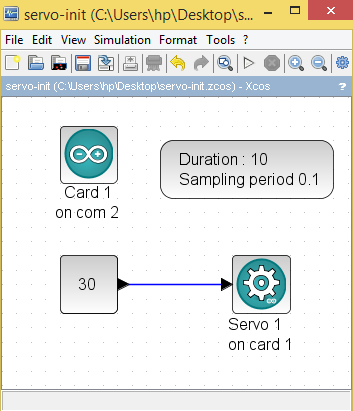
\includegraphics[width=\smfig]{\LocSERfig/servo-init.png}
          \caption[Rotating the servomotor by a fixed angle]{Rotating the
            servomotor by a fixed angle.  This is what one sees when
            \LocLEDscibrief{servo-init.zcos}, is invoked.}
          \label{fig:servo-init}
        \end{figure}
        
        We will next explain how to set the parameters for this simulation.
        To set value on any block, one needs to right click and open the
          {\tt Block Parameters} or double click.  The values for each block
        is tabulated in \tabref{tab:servo-init}.  All other parameters are to
        be left unchanged.
        \begin{table}
          \centering
          \caption{Parameters to rotate the servomotor by $30^\circ$}
          \label{tab:servo-init}
          \begin{tabular}{llc} \hline
            Name of the block & Parameter name             & Value     \\ \hline
            ARDUINO\_SETUP    & Identifier of Arduino Card & 1         \\
                              & Serial com port number     & 2\portcmd \\ \hline
            TIME\_SAMPLE      & Duration of acquisition(s) & 10        \\
                              & Sampling period(s)         & 0.1       \\ \hline
            SERVO\_WRITE\_SB  & Servo number               & 1         \\
                              & Arduino card number        & 1         \\ \hline
            CONST\_m          & Constant value             & 30        \\ \hline
          \end{tabular}
        \end{table}
        
  \item Next, we will rotate the servomotor by $90^\circ$ and bring it
        to $45^\circ$, all absolute values.  When the file required for this
        experiment is invoked, one gets the GUI as in
        \figref{fig:servo-reverse}.  In the caption of this figure, one can
        see where to locate the file.
        \begin{figure}
          \centering
          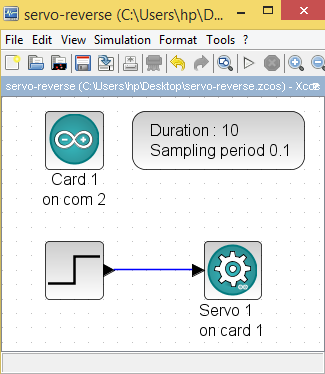
\includegraphics[width=\smfig]{\LocSERfig/servo-reverse.png}
          \caption[Rotating the servomotor forward and then
            reverse]{Rotating the servomotor forward and then reverse.  This
            is what one sees when \LocLEDscibrief{servo-reverse.zcos},
            is invoked.}
          \label{fig:servo-reverse}
        \end{figure}
        
        We will next explain how to set the parameters for this simulation.
        To set value on any block, one needs to right click and open the
          {\tt Block Parameters} or double click.  The values for each block
        is tabulated in \tabref{tab:servo-reverse}.  All other parameters
        are to be left unchanged.
        \begin{table}
          \centering
          \caption{Parameters to rotate the servomotor forward and reverse}
          \label{tab:servo-reverse}
          \begin{tabular}{llc} \hline
            Name of the block & Parameter name             & Value     \\ \hline
            ARDUINO\_SETUP    & Identifier of Arduino Card & 1         \\
                              & Serial com port number     & 2\portcmd \\ \hline
            TIME\_SAMPLE      & Duration of acquisition(s) & 10        \\
                              & Sampling period(s)         & 0.1       \\ \hline
            SERVO\_WRITE\_SB  & Servo number               & 1         \\
                              & Arduino card number        & 1         \\ \hline
            STEP\_FUNCTION    & Step time                  & 1         \\ 
                              & Initial value              & 90        \\
                              & Final value                & 45        \\ \hline
          \end{tabular}
        \end{table}
        
  \item Next, we will rotate the servomotor in increments of
        $20^\circ$.  When the file required for this
        experiment is invoked, one gets the GUI as in
        \figref{fig:servo-loop}.  In the caption of this figure, one can
        see where to locate the file.
        \begin{figure}
          \centering
          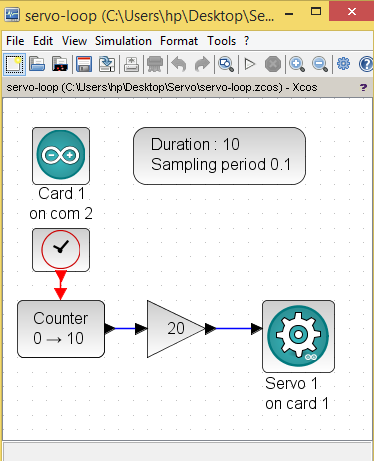
\includegraphics[width=\smfig]{\LocSERfig/servo-loop.png}
          \caption[Rotating the servomotor in increments of $20^\circ$]
          {Rotating the servomotor in increments of $20^\circ$.  This is what
            one sees when \LocLEDscibrief{servo-loop.zcos}, is invoked.}
          \label{fig:servo-loop}
        \end{figure}
        
        We will next explain how to set the parameters for this simulation.
        To set value on any block, one needs to right click and open the
          {\tt Block Parameters} or double click.  The values for each block
        is tabulated in \tabref{tab:servo-loop}.  {\tt Do on Overflow 0}
        means that we need to do nothing when there is an overflow.
        All other parameters are to be left unchanged.
        \begin{table}
          \centering
          \caption{Parameters to make the servomotor to sweep the entire
            range in increments}
          \label{tab:servo-loop}
          \begin{tabular}{llc} \hline
            Name of the block & Parameter name             & Value     \\ \hline
            ARDUINO\_SETUP    & Identifier of Arduino Card & 1         \\
                              & Serial com port number     & 2\portcmd \\ \hline
            TIME\_SAMPLE      & Duration of acquisition(s) & 10        \\
                              & Sampling period(s)         & 0.1       \\ \hline
            SERVO\_WRITE\_SB  & Servo number               & 1         \\ \hline
            CLOCK\_c          & Period                     & 1         \\
                              & Initialization time        & 0.1       \\ \hline
            Counter           & Minimum value              & 0         \\
                              & Maximum value              & 10        \\ 
                              & Rule                       & 1         \\ \hline
            GAINBLK           & Gain                       & 20        \\
                              & Do on overflow             & 0         \\ \hline
          \end{tabular}
        \end{table}
        
  \item Finally, we will use Xcos to rotate the servomotor as per the
        input received from the potentiometer.  When the file required for
        this experiment is invoked, one gets the GUI as in
        \figref{fig:servo-pot}.  In the caption of this figure, one can see
        where to locate the file.
        \begin{figure}
          \centering
          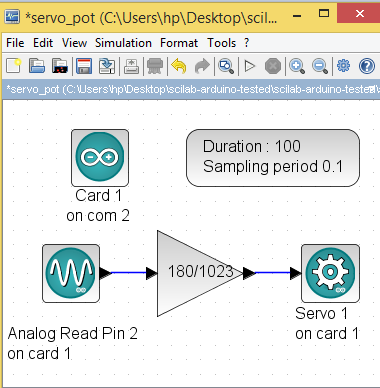
\includegraphics[width=\smfig]{\LocSERfig/servo-pot.png}
          \caption[Rotating the servomotor as suggested by the
            potentiometer]{Rotating the servomotor as suggested by the
            potentiometer.  This is what
            one sees when \LocLEDscibrief{servo-pot.zcos}, is invoked.}
          \label{fig:servo-pot}
        \end{figure}
        
        We will next explain how to set the parameters for this simulation.
        To set value on any block, one needs to right click and open the
          {\tt Block Parameters} or double click.  The values for each block
        is tabulated in \tabref{tab:servo-pot}.  All other parameters are to
        be left unchanged.  The {\tt ANALOG\_READ\_SB} block reads the value
        of potentiometer. Next, {\tt GAIN\_f} is used to convert the 
        potentiometer values into rotation angle by multiplying the values 
        with $180/1023$. 
        \begin{table}
          \centering
          \caption{Parameters to rotate the servomotor based on the input
            from the potentiometer}
          \label{tab:servo-pot}
          \begin{tabular}{llc} \hline
            Name of the block & Parameter name                 & Value     \\ \hline
            ARDUINO\_SETUP    & Identifier of Arduino Card     & 1         \\
                              & Serial com port number         & 2\portcmd \\ \hline
            TIME\_SAMPLE      & The duration of acquisition(s) & 100       \\
                              & Sampling period(s)             & 0.1       \\ \hline
            SERVO\_WRITE\_SB  & Servo number                   & 1         \\ \hline
            ANALOG\_READ\_SB  & Analog Pin                     & 2         \\ 
                              & Arduino card number            & 1         \\ \hline
            GAIN\_f           & Gain                           & 180/1023  \\ \hline
          \end{tabular}
        \end{table}
\end{enumerate}


\section{Controlling the servomotor through Python}
\subsection{Controlling the servomotor}
\label{sec:servo-py}
In this section, we discuss how to carry out the experiments of the
previous section from Python.  We will list the same four experiments,
in the same order. As mentioned earlier, the shield must be removed from 
the \arduino\ and the \arduino\ needs to be connected to the computer 
with a USB cable, as shown in \figref{arduino}. The reader should go through the instructions given in
\secref{sec:python-start} before getting started.

% In this section, we will carry out the servomotor control experiments
% using python.  We will follow the same order as in
% \secref{sec:servo-ard}.  We assume that the shield is attached to the
% \arduino\ board while doing these experiments.  They will work without
% the shield also, but in this case, our comments on colour LEDs
% lighting will not be applicable.  The reader should go through the
% instructions given in \secref{sec:py-start} before getting started.

\begin{enumerate}
  \item The first experiment makes the servomotor move by $30^\circ$. The code for this experiment is
        given in \pyref{py:servo-init}. As explained earlier in \secref{sec:light-py}, 
        we begin with importing necessary modules followed by setting up the serial port.
        Next, we attach the servomotor by issuing the command given below:
        \lstinputlisting[firstline=24,lastline=24]{\LocSERpycode/servo-init.py}
        As shown above, the servomotor is attached on board 1 (the first argument)
        to pin 1 (the second argument).  In the Python-Arduino toolbox discussed 
        in \secref{sec:python-toolbox}, pin 1 and pin 5 are connected. As a result, we connect the wire physically to
        pin 5, which is achieved by the shield as discussed in \secref{sec:servo-pril}.
        
        With this, we issue the command to move the servomotor by $30^\circ$ followed by a delay of 
        1 second:
        \lstinputlisting[firstline=25,lastline=26]
        {\LocSERpycode/servo-init.py}
        At last, we  detach the servomotor followed by closing the serial port. 
        
        Once this code is executed, the servomotor would move by
        $30^\circ$, as commanded.  What happens if this code is executed
        once again?  The motor will not move at all.  What is the reason?
        Recall that what we assign to the motor are absolute positions, with
        respect to a fixed origin.  As a result, there will be no change at
        all. 
        
  \item In the second experiment, we move the servomotor by $90^\circ$ in the
        forward direction and $45^\circ$ in the reverse direction.  This
        code is given in \pyref{py:servo-reverse}.  In this code, 
        we have added a delay of 1 second between the two instances of 
        moving the servomotor: 
        \lstinputlisting[firstline=25,lastline=27]
        {\LocSERpycode/servo-reverse.py}
        What is the reason behind this delay?  If the delay were not
        there, the motor will move only by the net angle of $90-45 = 45$
        degrees.  The reader should verify this by commenting on the delay
        command. 
        
        % In \sciref{sci:servo-reverse}, we make the servomotor rotate
        % to $90^\circ$, wait for a second and go to $45^\circ$.  As mentioned
        % earlier, the angles are absolute with respect to a fixed reference
        % point and not relative.  
        
        
  \item In the third experiment, we move the motor in increments of
        $20^\circ$.  This is achieved by the {\tt for} loop, as in
        \pyref{py:servo-loop}. The code helps the motor move in steps of $20^\circ$ all
        the way to $180^\circ$.  
        
  \item Finally, in the last experiment, we read the potentiometer value
        from the shield and use it to drive the servomotor, see
        \pyref{py:servo-pot}.  The resistance of the potentiometer is
        represented in 10 bits.  As a result, the resistance value could be
        any one of 1024 values, from 0 to 1023.  This entire range is
        mapped to $180^\circ$, as shown below:
        \lstinputlisting[firstline=27,lastline=29]
        {\LocSERpycode/servo-pot.py}
        By rotating the potentiometer, one can make
        the motor move by different amounts.
        
        As mentioned in \chapref{potmeter}, the potentiometer on the shield is connected 
        to analog pin 2 on \arduino. Through this pin, the resistance of the potentiometer, in the range of 0 to 1023,
        depending on its position, is read.  Thus, by rotating the
        potentiometer, we make different values appear on pin 2.  This value
        is used to move the servo.  For example, if the resistance is half
        of the total, the servomotor will go to $90^\circ$ and so on.  The
        servomotor stops for 500 milliseconds after every move.  The loop is
        executed for 50 iterations. During this period, the servomotor keeps moving as dictated by the
        resistance of the potentiometer. While running this experiment, the readers 
        must rotate the knob of the potentiometer by a fixed amount and observe 
        the change in the position (or angle) of the servomotor.   
        % In the first experiment, we will learn how to drive the servomotor motor
        % from Python. The code for this experiment is 
        % given in  \pyref{py:servo-init}. 
        
        % The first experiment makes the servomotor move by $30^\circ$,
        %       the code for which is given in \pyref{py:servo-init}.
        %       It first opens com port 2 in \arduino\ card number 1 with baud rate
        %       of 115200.  If the port opening is unsuccessful {\tt ok} will not be
        %       0 and the program terminates, asking the user to correct the
        %       problem.  Else If the port opening is successful, {\tt ok} will be 0
        %       and the program proceeds.  In Line number 3 of the code, \ie\
        %       \lstinputlisting[firstline=3,lastline=3]{\LocSERpycode/servo-init.py}
        %       we say that the servomotor is attached on board 1 (the first entry)
        %       to pin 1 (the second entry).  In the \scilab\ toolbox, pin 1 and pin
        %       9 are connected and as a result, we connect the wire physically to
        %       pin 9.  Similarly, pins 2 and 10 are connected through the
        %       \scilab\ toolbox.
        
        % \item In \sciref{py:servo-reverse}, we make the servomotor rotate
        %       to $90^\circ$, wait for a second and go to $45^\circ$.  As mentioned
        %       earlier, the angles are absolute with respect to a fixed reference
        %       point and not relative.  
        
        % \item In the next experiment, we rotate the servomotor in discrete
        %       steps of $20^\circ$.  This is achieved by multiplying $20^\circ$ by
        %       an integer {\tt i}, which varies from 0 to 10.  Once the maximum
        %       angle reaches $180^\circ$, it stops.  
        
        % \item Finally, in the last experiment, we position the servomotor
        %       through the potentiometer in the code \pyref{py:servo-pot}.  As we
        %       rotate the potentiometer, the servomotor's angle also changes.  The
        %       potentiometer value is read through pin 2, in line number 5, as
        %       below:
        %       \lstinputlisting[firstline=5,lastline=5]{\LocSERpycode/servo-pot.py}
        %       This value is mapped into a value between 0 and $180^\circ$ by
        %       multiplying with $180/1023$ in line 6:
        %       \lstinputlisting[firstline=6,lastline=6]{\LocSERpycode/servo-pot.py}
        %       The {\tt floor} function gets the integer part of the number by
        %       truncation.  This is the angle by which the potentiometer is to be
        %       moved.  Truncation is a not a crucial calculation, however.  In
        %       every iteration, the servomotor's position is calculated, and placed
        %       for half a second.  This loop is iterated upon 5,000 times.
\end{enumerate}

\subsection{Python Code}
\lstset{style=mystyle}
\label{sec:servo-python-code}
\addtocontents{pyd}{\protect\addvspace{\codclr}}

\begin{pycode}
  \pcaption{Rotating the servomotor to a specified degree} {Rotating
    the servomotor to a specified degree.  Available at
    \LocSERpybrief{servo-init.py}.}
  \label{py:servo-init}
  \lstinputlisting{\LocSERpycode/servo-init.py}
\end{pycode}

\begin{pycode}
  \pcaption{Rotating the servomotor to a specified degree and
    reversing} {Rotating
    the servomotor to a specified degree and reversing.  Available at
    \LocSERpybrief{servo-reverse.py}.}
  \label{py:servo-reverse}
  \lstinputlisting{\LocSERpycode/servo-reverse.py}
\end{pycode}

\begin{pycode}
  \pcaption{Rotating the servomotor in steps of $20^\circ$}{Rotating
    the servomotor in steps of $20^\circ$.  Available at 
    \LocSERpybrief{servo-loop.py}.}
  \label{py:servo-loop}
  \lstinputlisting{\LocSERpycode/servo-loop.py}
\end{pycode}

\begin{pycode}
  \pcaption{Rotating the servomotor to a degree specified by the
    potentiometer} {Rotating the servomotor to a degree specified by
    the potentiometer.  Available at \LocSERpybrief{servo-pot.py}.}
  \label{py:servo-pot}
  \lstinputlisting{\LocSERpycode/servo-pot.py}
\end{pycode}

\section{Controlling the servomotor through Julia}
\subsection{Controlling the servomotor}
\label{sec:servo-julia}
In this section, we discuss how to carry out the experiments of the
previous section from Julia.  We will list the same four experiments,
in the same order. As mentioned earlier, the shield must be removed from 
the \arduino\ and the \arduino\ needs to be connected to the computer 
with a USB cable, as shown in \figref{arduino}. 
The reader should go through the instructions given in \secref{sec:julia-start} before getting started.


\begin{enumerate}
  \item The first experiment makes the servomotor move by $30^\circ$. The code for this experiment is
        given in \juliaref{julia:servo-init}. As explained earlier in \secref{sec:light-julia}, 
        we begin with importing necessary modules followed by setting up the serial port.
        Next, we attach the servomotor by issuing the command given below:
        \lstinputlisting[firstline=5,lastline=5]{\LocSERjuliacode/servo-init.jl}
        As shown above, the servomotor is attached on the serial port (the first argument)
        to pin 1 (the second argument).  In the Julia-Arduino toolbox discussed 
        in \secref{sec:julia-toolbox}, pin 1 and pin 5 are connected. As a result, we connect the wire physically to
        pin 5, which is achieved by the shield as discussed in \secref{sec:servo-pril}.
        
        With this, we issue the command to move the servomotor by $30^\circ$ followed by a delay of 
        1 second:
        \lstinputlisting[firstline=6,lastline=6]
        {\LocSERjuliacode/servo-init.jl}
        At last, we  detach the servomotor followed by closing the serial port. 
        
        Once this code is executed, the servomotor would move by
        $30^\circ$, as commanded.  What happens if this code is executed
        once again?  The motor will not move at all.  What is the reason?
        Recall that what we assign to the motor are absolute positions, with
        respect to a fixed origin.  As a result, there will be no change at
        all. 
        
  \item In the second experiment, we move the servomotor by $90^\circ$ in the
        forward direction and $45^\circ$ in the reverse direction.  This
        code is given in \juliaref{julia:servo-reverse}.  As mentioned
        earlier, the angles are absolute with respect to a fixed reference
        point and not relative.   In this code, 
        we have added a delay of 1 second between the two instances of 
        moving the servomotor: 
        \lstinputlisting[firstline=6,lastline=8]
        {\LocSERjuliacode/servo-reverse.jl}
        What is the reason behind this delay?  If the delay were not
        there, the motor will move only by the net angle of $90-45 = 45$
        degrees.  The reader should verify this by commenting on the delay
        command. 
        
        
  \item In the third experiment, we move the motor in increments of
        $20^\circ$.  This is achieved by the {\tt for} loop, as in
        \juliaref{julia:servo-loop}. The code helps the motor move in steps of $20^\circ$ all
        the way to $180^\circ$.  
        
  \item Finally, in the last experiment, we read the potentiometer value
        from the shield and use it to drive the servomotor, see
        \juliaref{julia:servo-pot}.  The resistance of the potentiometer is
        represented in 10 bits.  As a result, the resistance value could be
        any one of 1024 values, from 0 to 1023.  This entire range is
        mapped to $180^\circ$, as shown below:
        \lstinputlisting[firstline=7,lastline=10]
        {\LocSERjuliacode/servo-pot.jl}
        By rotating the potentiometer, one can make
        the motor move by different amounts.
        
        As mentioned in \chapref{potmeter}, the potentiometer on the shield is connected 
        to analog pin 2 on \arduino. Through this pin, the resistance of the potentiometer, in the range of 0 to 1023,
        depending on its position, is read.  Thus, by rotating the
        potentiometer, we make different values appear on pin 2.  This value
        is used to move the servo.  For example, if the resistance is half
        of the total, the servomotor will go to $90^\circ$ and so on.  The
        servomotor stops for 500 milliseconds after every move.  The loop is
        executed for 50 iterations. During this period, the servomotor keeps moving as dictated by the
        resistance of the potentiometer. While running this experiment, the readers 
        must rotate the knob of the potentiometer by a fixed amount and observe 
        the change in the position (or angle) of the servomotor.   
        
        % The {\tt floor} function gets the integer part of the number by
        % truncation.  This is the angle by which the potentiometer is to be
        % moved.  Truncation is a not a crucial calculation, however.  In
        % every iteration, the servomotor's position is calculated, and placed
        % for half a second.  This loop is iterated upon 500 times.
\end{enumerate}

\subsection{Julia Code}
\lstset{style=mystyle}
\label{sec:servo-julia-code}
\addtocontents{juliad}{\protect\addvspace{\codclr}}

\begin{juliacode}
  \jcaption{Rotating the servomotor to a specified degree} {Rotating
    the servomotor to a specified degree.  Available at
    \LocSERjuliabrief{servo-init.jl}.}
  \label{julia:servo-init}
  \lstinputlisting{\LocSERjuliacode/servo-init.jl}
\end{juliacode}

\begin{juliacode}
  \jcaption{Rotating the servomotor to a specified degree and
    reversing} {Rotating
    the servomotor to a specified degree and reversing.  Available at
    \LocSERjuliabrief{servo-reverse.jl}.}
  \label{julia:servo-reverse}
  \lstinputlisting{\LocSERjuliacode/servo-reverse.jl}
\end{juliacode}

\begin{juliacode}
  \jcaption{Rotating the servomotor in steps of $20^\circ$}{Rotating
    the servomotor in steps of $20^\circ$.  Available at 
    \LocSERjuliabrief{servo-loop.jl}.}
  \label{julia:servo-loop}
  \lstinputlisting{\LocSERjuliacode/servo-loop.jl}
\end{juliacode}

\begin{juliacode}
  \jcaption{Rotating the servomotor to a degree specified by the
    potentiometer} {Rotating the servomotor to a degree specified by
    the potentiometer.  Available at \LocSERjuliabrief{servo-pot.jl}.}
  \label{julia:servo-pot}
  \lstinputlisting{\LocSERjuliacode/servo-pot.jl}
\end{juliacode}

\section{Controlling the servomotor through OpenModelica}
\subsection{Controlling the servomotor}
\label{sec:servo-OpenModelica}
In this section, we discuss how to carry out the experiments of the
previous section from OpenModelica.  We will list the same four experiments,
in the same order.  As mentioned earlier, the shield must be removed from 
the \arduino\ and the \arduino\ needs to be connected to the computer 
with a USB cable, as shown in \figref{arduino}. The reader should go through the instructions given in
\secref{sec:OpenModelica-start} before getting started.

\begin{enumerate}

  \item The first experiment makes the servomotor move by $30^\circ$. The code for this experiment is
        given in \OpenModelicaref{OpenModelica:servo-init}. As explained earlier in \secref{sec:light-OpenModelica}, 
        we begin with importing the two packages: Streams and SerialCommunication followed 
        by setting up the serial port. Next, we attach the servomotor by issuing the command given below:
        
        \lstinputlisting[firstline=13,lastline=13]{\LocSEROpenModelicacode/servo-init.mo}
        As shown above, the servomotor is attached on board 1 (the first argument)
        to pin 1 (the second argument).  In the OpenModelica-Arduino toolbox discussed 
        in \secref{sec:load-om-toolbox}, pin 1 and pin 5 are connected. As a result, we connect the wire physically to
        pin 5, which is achieved by the shield as discussed in \secref{sec:servo-pril}.
        
        With this, we issue the command to move the servomotor by $30^\circ$ followed by a delay of 
        1 second:
        \lstinputlisting[firstline=14,lastline=14]
        {\LocSEROpenModelicacode/servo-init.mo}
        At last, we  detach the servomotor followed by closing the serial port. 
        
        Once this code is executed, the servomotor would move by
        $30^\circ$, as commanded.  What happens if this code is executed
        once again?  The motor will not move at all.  What is the reason?
        Recall that what we assign to the motor are absolute positions, with
        respect to a fixed origin.  As a result, there will be no change at
        all. 
        
  \item In the second experiment, we move the servomotor by $90^\circ$ in the
        forward direction and $45^\circ$ in the reverse direction.  This
        code is given in \OpenModelicaref{OpenModelica:servo-reverse}.  As mentioned
        earlier, the angles are absolute with respect to a fixed reference
        point and not relative.   In this code, 
        we have added a delay of 1000 milliseconds between the two instances of 
        moving the servomotor: 
        \lstinputlisting[firstline=15,lastline=17]
        {\LocSEROpenModelicacode/servo-reverse.mo}
        What is the reason behind this delay?  If the delay were not
        there, the motor will move only by the net angle of $90-45 = 45$
        degrees.  The reader should verify this by commenting on the delay
        command. 
        
        
  \item In the third experiment, we move the motor in increments of
        $20^\circ$.  This is achieved by the {\tt for} loop, as in
        \OpenModelicaref{OpenModelica:servo-loop}. The code helps the motor move in steps of $20^\circ$ all
        the way to $180^\circ$.  
        
  \item Finally, in the last experiment, we read the potentiometer value
        from the shield and use it to drive the servomotor, see
        \OpenModelicaref{OpenModelica:servo-pot}.  The resistance of the potentiometer is
        represented in 10 bits.  As a result, the resistance value could be
        any one of 1024 values, from 0 to 1023.  This entire range is
        mapped to $180^\circ$, as shown below:
        \lstinputlisting[firstline=17,lastline=19]
        {\LocSEROpenModelicacode/servo-pot.mo}
        By rotating the potentiometer, one can make
        the motor move by different amounts.
        
        As mentioned in \chapref{potmeter}, the potentiometer on the shield is connected 
        to analog pin 2 on \arduino. Through this pin, the resistance of the potentiometer, in the range of 0 to 1023,
        depending on its position, is read.  Thus, by rotating the
        potentiometer, we make different values appear on pin 2.  This value
        is used to move the servo.  For example, if the resistance is half
        of the total, the servomotor will go to $90^\circ$ and so on.  The
        servomotor stops for 500 milliseconds after every move.  The loop is
        executed for 50 iterations. During this period, the servomotor keeps moving as dictated by the
        resistance of the potentiometer. While running this experiment, the readers 
        must rotate the knob of the potentiometer by a fixed amount and observe 
        the change in the position (or angle) of the servomotor. 
        
\end{enumerate}

\subsection{OpenModelica Code}
\lstset{style=mystyle}
\label{sec:servo-OpenModelica-code}
Unlike other code files, the code/ model for running experiments using OpenModelica are 
available inside the OpenModelica-Arduino toolbox, as explained in \secref{sec:load-om-toolbox}.
Please refer to \figref{om-examples-toolbox} to know how to locate the experiments. 

\addtocontents{OpenModelicad}{\protect\addvspace{\codclr}}

\begin{OpenModelicacode}
  \mcaption{Rotating the servomotor to a specified degree} {Rotating
    the servomotor to a specified degree. Available at Arduino -> 
    SerialCommunication -> Examples -> servo -> servo\_init.}
  \label{OpenModelica:servo-init}
  \lstinputlisting{\LocSEROpenModelicacode/servo-init.mo}
\end{OpenModelicacode}

\begin{OpenModelicacode}
  \mcaption{Rotating the servomotor to a specified degree and
    reversing} {Rotating
    the servomotor to a specified degree and reversing.  Available at Arduino -> 
    SerialCommunication -> Examples -> servo -> servo\_reverse.}
  \label{OpenModelica:servo-reverse}
  \lstinputlisting{\LocSEROpenModelicacode/servo-reverse.mo}
\end{OpenModelicacode}

\begin{OpenModelicacode}
  \mcaption{Rotating the servomotor in steps of $20^\circ$}{Rotating
    the servomotor in steps of $20^\circ$.  Available at Arduino -> 
    SerialCommunication -> Examples -> servo -> servo\_loop.}
  \label{OpenModelica:servo-loop}
  \lstinputlisting{\LocSEROpenModelicacode/servo-loop.mo}
\end{OpenModelicacode}

\begin{OpenModelicacode}
  \mcaption{Rotating the servomotor to a degree specified by the
    potentiometer} {Rotating the servomotor to a degree specified by
    the potentiometer.  Available at Arduino -> 
    SerialCommunication -> Examples -> servo -> servo\_pot.}
  \label{OpenModelica:servo-pot}
  \lstinputlisting{\LocSEROpenModelicacode/servo-pot.mo}
\end{OpenModelicacode}
